\subsection{Ensemble methods}

\vspace{0.2cm}
\noindent
\textbf{Random Forest \& Bagging}

We improved the tree-based models using bagging with 500 trees and random forest, selecting the best number of predictors (\textit{m}) from the full set of \textit{p} predictors.

In \Fig~\ref{fig:m_best_for_500_plot} we can see the trend of the test and the out-of-bag error rates as \textit{m} increases.

\begin{figure}[h]
	\centering
	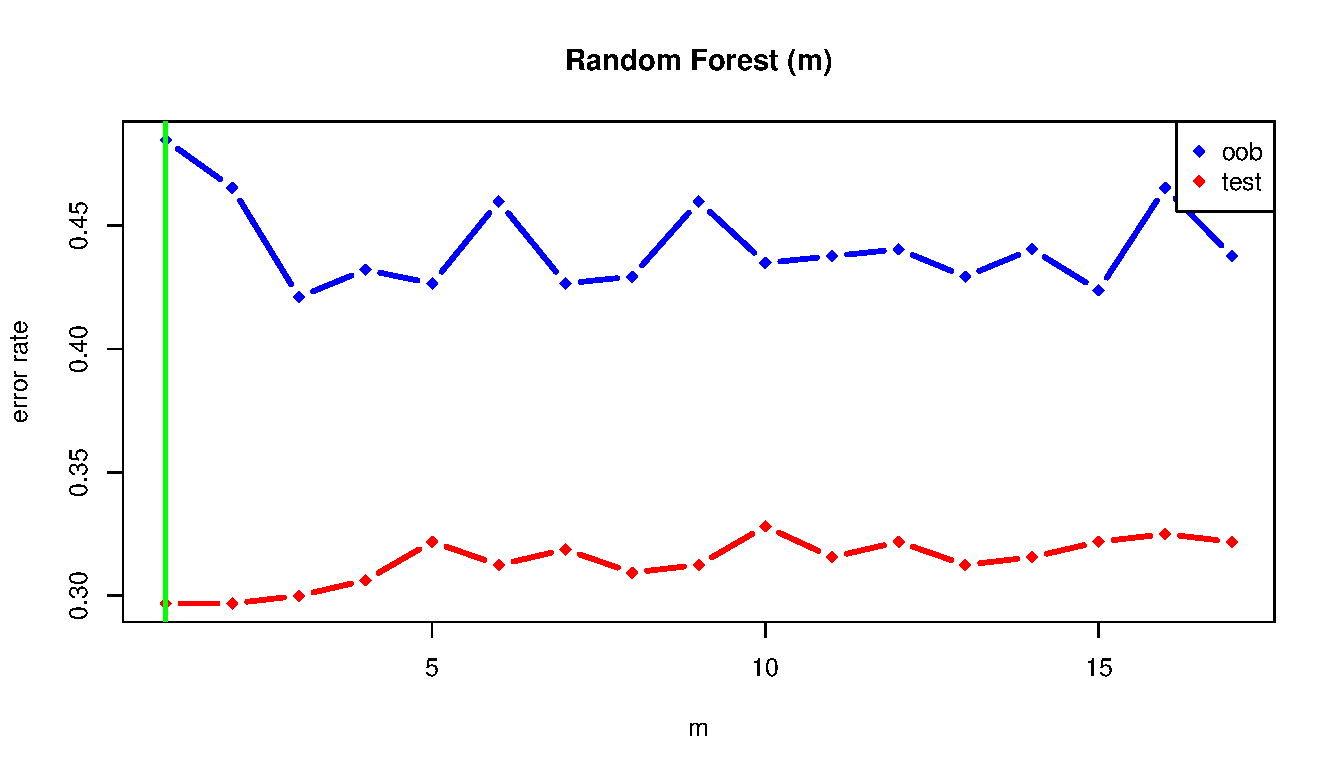
\includegraphics[width=0.5\linewidth]{ImageFiles/Classification/Trees/m_best_for_500_plot}
	\caption{Test and out-of-bag trends}
	\label{fig:m_best_for_500_plot}
\end{figure}

Once the best \textit{m} value for the random forest was obtained, we compared the bagging model with the random forest model using that particular value of \textit{m}, while keeping all other parameters the same.
In \Fig~\ref{fig:vs_bagg_for_500_plot} we can see that random forest performs slightly better than bagging.

\begin{figure}[H]
	\centering
	\begin{subfigure}{.3\textwidth}
		\centering
		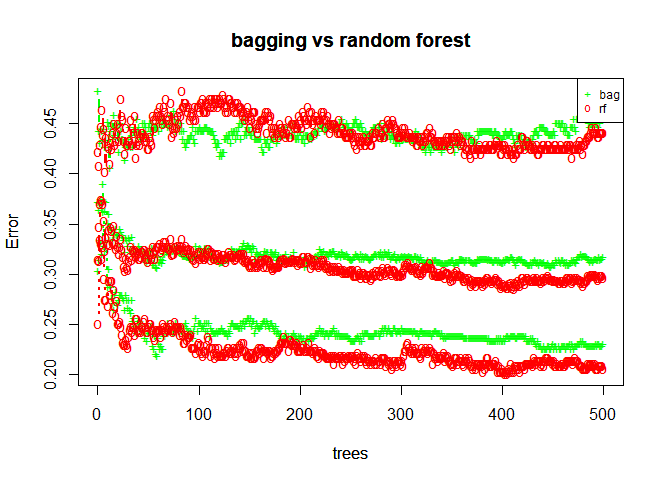
\includegraphics[width=\linewidth]{ImageFiles/Classification/Trees/vs_bagg_for_500_plot}
		\caption{Bagging and random forest comparison.}
		\label{fig:vs_bagg_for_500_plot}
	\end{subfigure}%
	\hfill
	\begin{subfigure}{.3\textwidth}
		\centering
		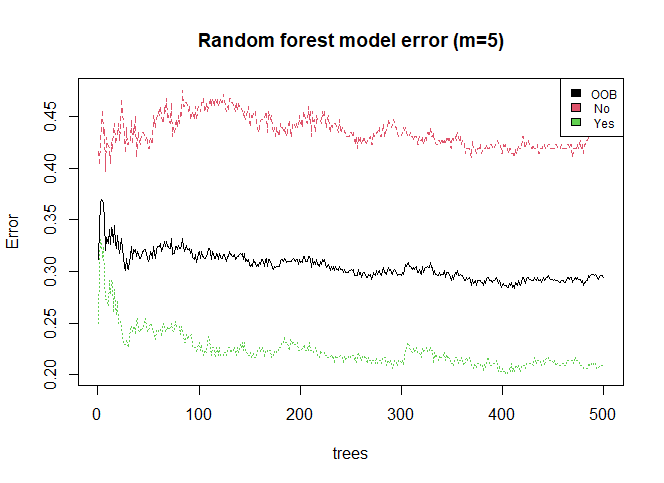
\includegraphics[width=\linewidth]{ImageFiles/Classification/Trees/best_for_500_plot}
		\caption{Random forest method plot.}
		\label{fig:best_for_500_plot}
	\end{subfigure}%
	\hfill
	\begin{subfigure}{.3\textwidth}
		\centering
		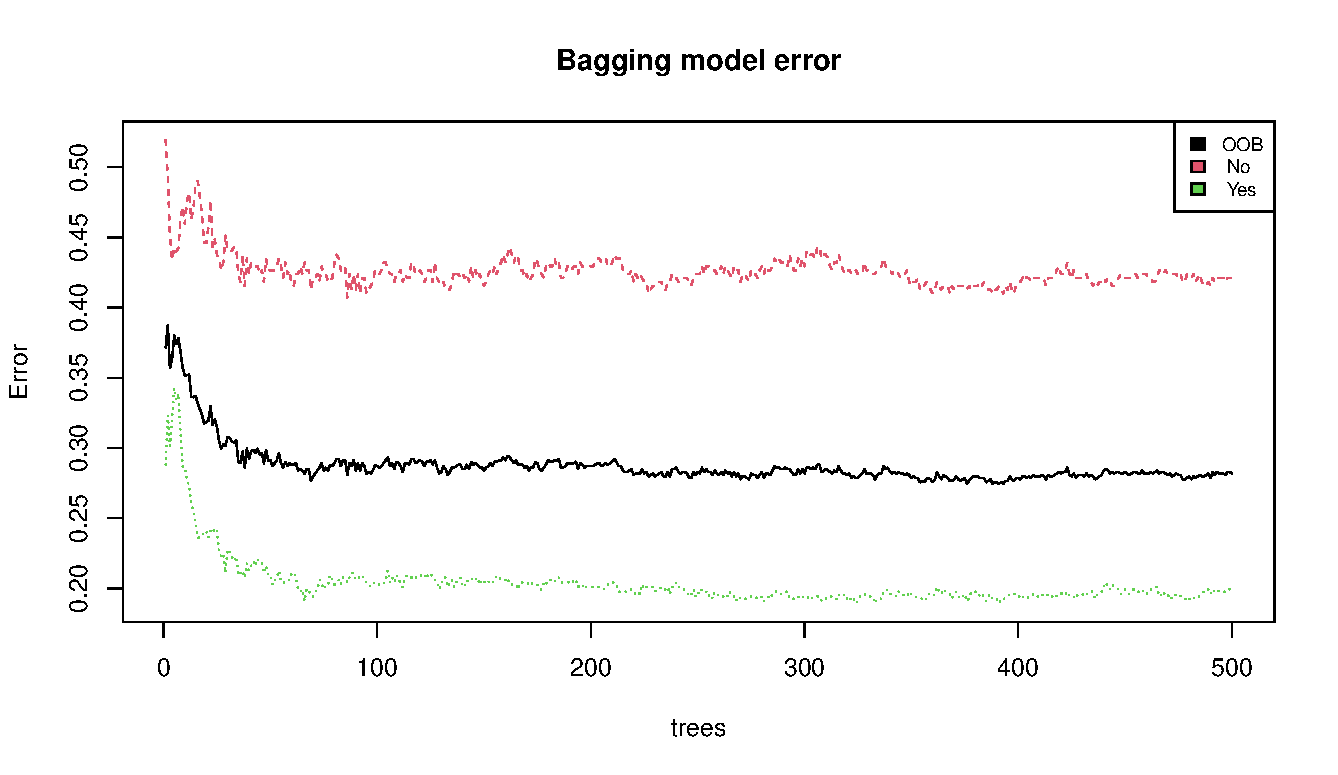
\includegraphics[width=\linewidth]{ImageFiles/Classification/Trees/bagg_500_plot}
		\caption{Bagging method plot.}
		\label{fig:bagg_500_plot}
	\end{subfigure}
	\caption{Random Forest vs Bagging.}
	\label{fig:RFvsB}
\end{figure}

An overall summary of the importance of each predictor is obtained by using RSS (\textit{"Residual Sum of Squares"}). In \Fig~\ref{fig:best_for_500_var_imp_plot} and \Fig~\ref{fig:bagg_500_var_imp_plot} we can see the importance of each variable in the models.

\begin{figure}[h]
	\centering
	\begin{subfigure}{.5\textwidth}
		\centering
		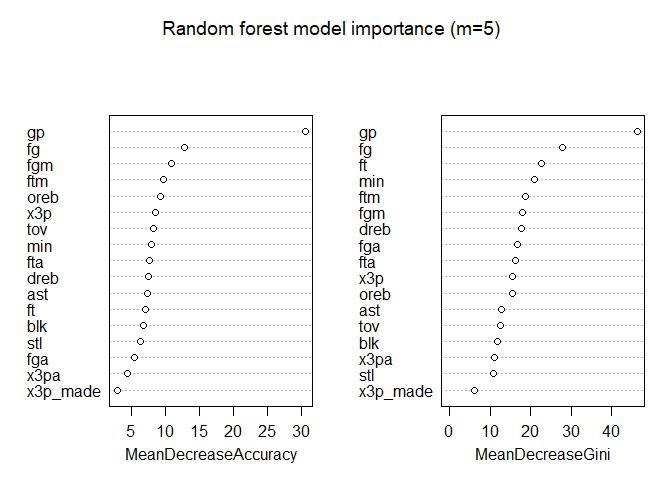
\includegraphics[width=0.5\linewidth]{ImageFiles/Classification/Trees/best_for_500_var_imp_plot}
		\caption{Random forest important variables.}
		\label{fig:best_for_500_var_imp_plot}
	\end{subfigure}%
	\hfill
	\begin{subfigure}{.5\textwidth}
		\centering
		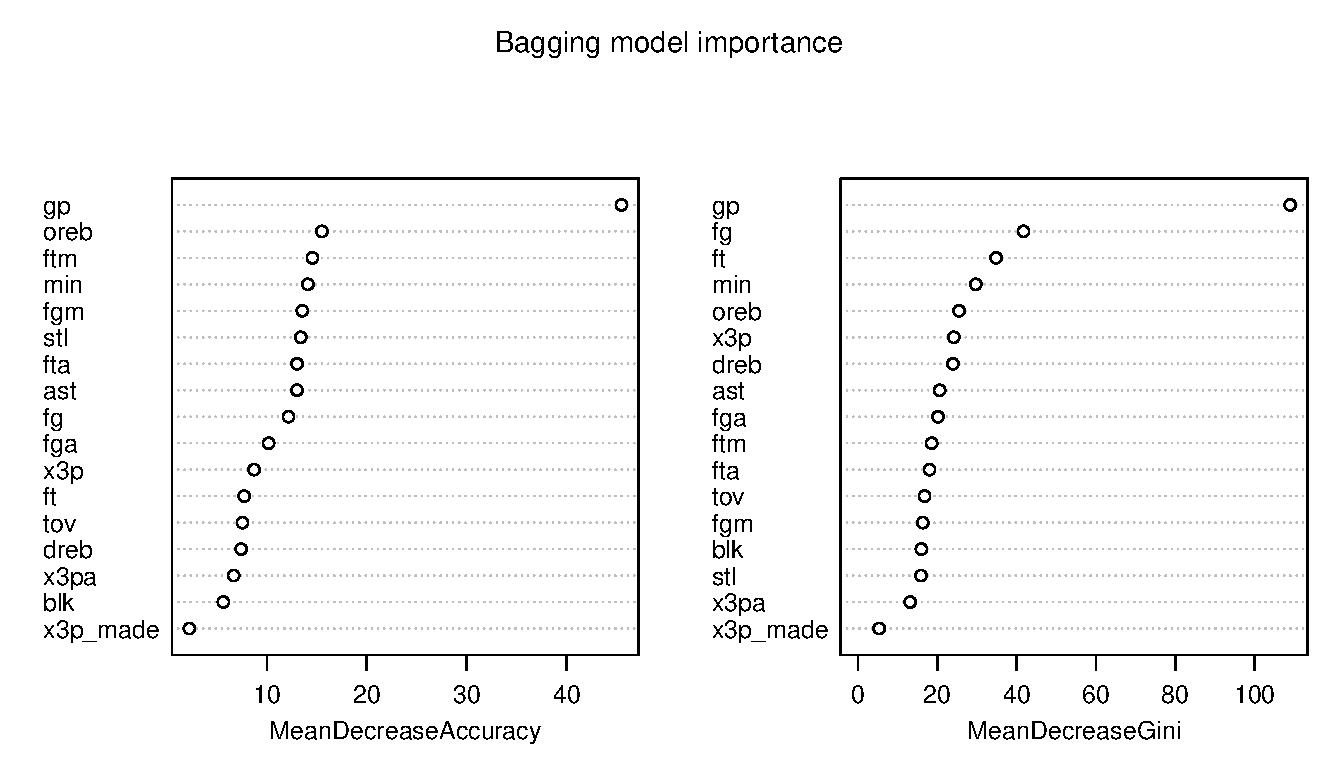
\includegraphics[width=0.5\linewidth]{ImageFiles/Classification/Trees/bagg_500_var_imp_plot}
		\caption{Bagging important variable.}
		\label{fig:bagg_500_var_imp_plot}
	\end{subfigure}
	\caption{Important variables.}
	\label{fig:ImpVar}
\end{figure}

\noindent
As in the classification trees, the \textit{gp} regressor resulted to be the most important one.

\vspace{0.2cm}
\noindent
\textbf{Boosting}

Since the main goal of this section is to find the model that best explain our data, we tried to improve the performance by using \textit{boosting} in conjunction with cross-validation, even at the cost of losing interpretability. 

Many small trees were used with $\lambda = 0.001$. \Fig~\ref{fig:boost_4_rel_inf} shows the importance of each variable in the dataset given by the boosting technique.

\begin{figure}[H]
	\centering
	\begin{subfigure}{.5\textwidth}
		\centering
		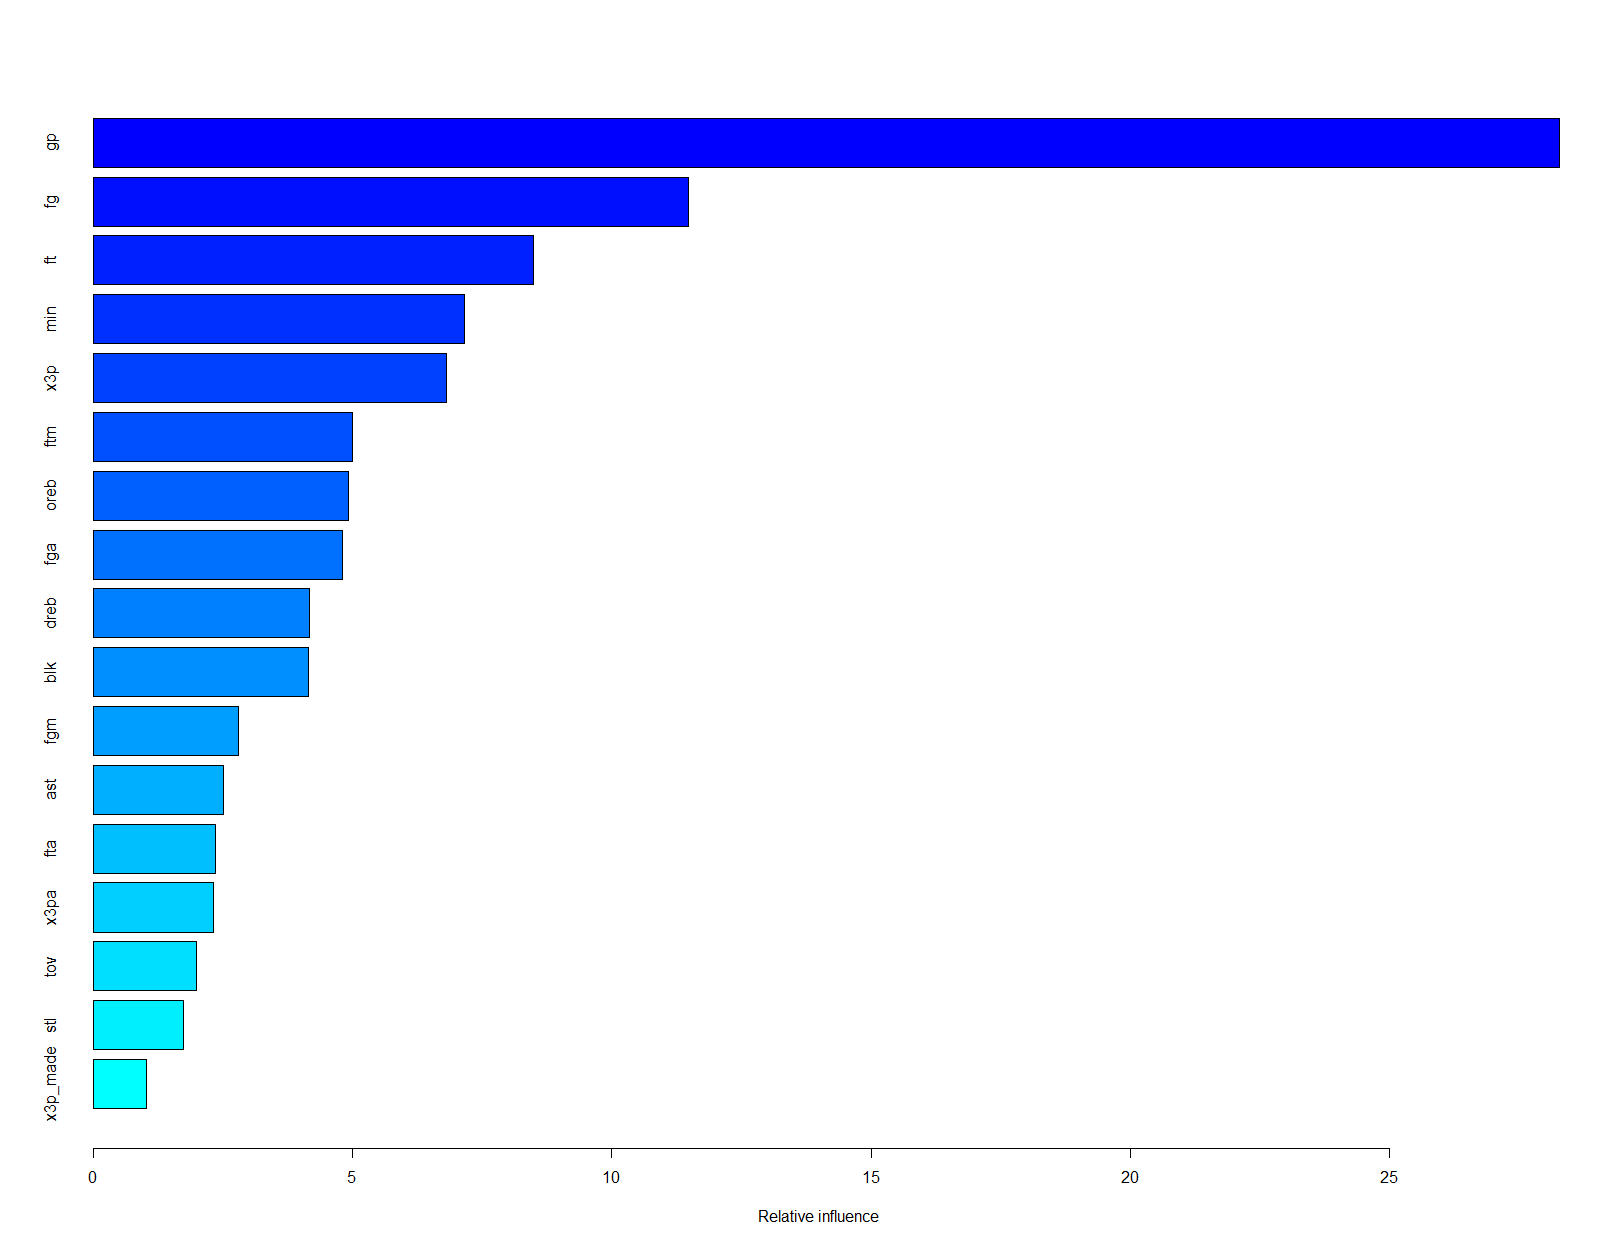
\includegraphics[width=0.6\linewidth]{ImageFiles/Classification/Trees/boost_4_rel_inf}
		\caption{Boosting relative influence.}
		\label{fig:boost_4_rel_inf}
	\end{subfigure}%
	\hfill
	\begin{subfigure}{.5\textwidth}
		\centering
		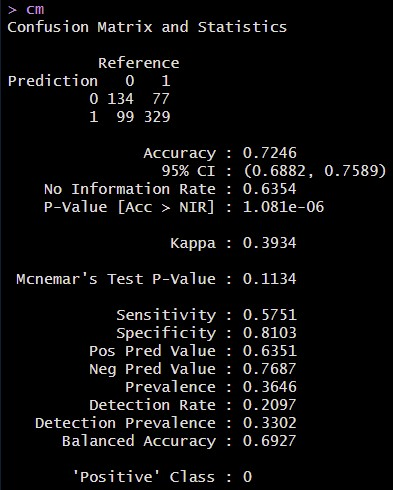
\includegraphics[width=0.4\linewidth]{ImageFiles/Classification/Trees/boost_4_conf_mat}
		\caption{Boosting confusion matrix.}
		\label{fig:boost_4_conf_mat}
	\end{subfigure}
	\caption{Boosting results.}
	\label{BoostRes}
\end{figure}

As with the previous models, the most significant regressor is still \textit{gp}. However, based on the confusion matrix in \Fig~\ref{fig:boost_4_conf_mat}, it results that there is no improvement in accuracy. Therefore, using \textit{boosting} is not recommended, since it would just lead to interpretability loss.

